\documentclass[a4paper]{report}
\usepackage{tikz}
\usepackage{ulem}
\usepackage{minted}
\usepackage{hyperref}
\usepackage{graphicx}
\usepackage{fontspec}
\usepackage{tabulary}
\usetikzlibrary{shapes.geometric, arrows}
\usemintedstyle{vs}
\graphicspath{ {./images/} {./graphs/} }
\setlength{\parindent}{0pt}
\setlength{\parskip}{1em}
\title{A Level Programming Project Report}
\author{Junrong Chen}
\date{\today}

\begin{document}
\maketitle
\tableofcontents
\clearpage
\chapter{Analysis}

\section{Problem Identification}

A Level Computer Science students need to learn many algorithms and data structures during the course. In the final exam, they need to write pseudocode to solve computational questions. Many students find it is hard to achieve a high score on those questions due to the lack of efficient training. The general method used by students to learn and revise for Computer Science is to attempt and self-mark past paper questions. This works well for ordinary questions. However, for the algorithm questions, different students may produce completely different code solutions. This makes their self-marking very unreliable. It is also too much work for the teacher to mark their solutions one by one. So, in the end, students do not know whether they get things right, and teachers do not know how the students perform and how they can help, especially in this lockdown online learning era where no direct contact between teachers and students is possible.

Both the students and the teachers are looking for a more efficient method to learn and practice.

\section{Stakeholders}

There are two types of stakeholders, Computer Science teachers and Computer Science students.

\subsection{Computer Science teachers}

Computer Science teachers find it is difficult to monitor their students' ability to design and implement algorithms, so they cannot provide efficient help to their students. This software allows them to create coding questions and send them to the students. After the students hand their solutions back, the software will automatically mark their answers and provide detailed statistical data with simple visualisations. This helps the teachers saving a lot of time and allows them to help the students better.

The stakeholder is Mr. Grimwood, who is an experienced A Level Computer Science teacher who teaches a Year 12 CS group and a Year 13 CS group.

\subsection{Computer Science students}

Computer Science students find that they tend to lose mark on the algorithms coding questions, so they want more practice. But unlike ordinary questions, they may take a completely different approach towards the questions comparing to the mark scheme, so they do not know whether they get it correct. Students may also think they have got things right, but actually, they have made some mistakes. The software provides a free practice space that automatically marks their solutions and points out their mistakes in real-time. So the students can learn and revise more efficiently.

The stakeholders are Timofei and PCloud, they are both Year 13 students studying A Level Computer Science.

\section{Why it is suited to a computational solution}

The original problem, `understand and mark a student's answer' is a very difficult question for a computer to solve. But I transform the question into `compare the output of the students' code with pre-generated test cases', which makes the problem solvable using a computational method, since a computer is good at `executing a piece of code' and `comparing two strings'. This approach solves the `marking' question from another angle, and makes the question suited to a computational solution.

\section{Solve by computational methods}

\subsection{Thinking abstractly}

In reality, students use pens and paper to write their code solutions. This can be simplified into a code editor, and the students can use their keyboards to type in the code. In this way, no `text scanning' or `handwriting recognization' is needed which makes the design and programming much easier. The code editor will also provide a better user experience. Features such as syntax highlighting cannot exist on paper but are possible in a code editor.

In reality, the students' answer is sent to a teacher to mark it against the mark scheme. The teacher needs to read the code line by line and check whether it is correct. This process is abstracted into a judger that marks the code against pre-generated test cases, which transforms a problem that originally cannot be solved by computational method into one which is very easy to be solved by a computer while saving time and costs. When creating a new question, instead of creating a mark scheme for marking, the teacher needs to provide test cases with the correct input and expected output. The judger will run the students' submissions with the input and check whether their output matches the expected one.

\subsection{Thinking ahead}

For teachers, the software requires them to enter questions and test cases. A question editor containing input boxes is needed for this purpose. For students, the software requires them to enter their code solutions. A code editor is needed for this purpose. A relational database is need to store all the data. For all users, the software requires input data from mouse and keyboard to navigate between different windows and menus. Users will also need a monitor for the program to display all the information and outputs.

\subsection{Thinking procedurally and decomposition}

The program can be decomposed into several parts. Each part can be designed and maintained individually. Different components can interact with each other using custom APIs.

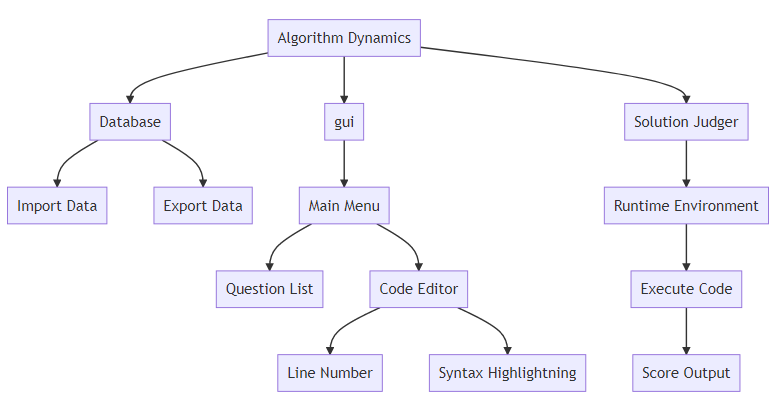
\includegraphics[width=\linewidth]{decomposition}

\subsection{Thinking concurrently}

When judging the students' solution, many test cases can be executed at the same time to reduce the judging time. The number of parallel judgers need to be set carefully based on the user's hardware. Running too few test cases concurrently may result in a very long judging time while running too many test cases at the same time may use up computing resources and cause issues.

\section{Interview}

\subsection{Design the interview}

\subsubsection{Interview for teachers}

\begin{enumerate}
    \item Do you find your students tend to lose marks on programming questions in exams?
    \item Do you find marking the programming question takes a lot of time and effort?
    \item Compare to the knowledge-based Computer System section, do you find it is more difficult to monitor students' skill level on the Algorithm and Programming section?
    \item Have you ever heard about some online programming platforms?
    \item Have you ever tried some of the online programming platforms?
    \item If yes, what do you think about these platforms? Have you ever considered to use them for teaching and training?
    \item Do you think a similar solution can help improve the efficienty of learning and training?
    \item If no, do you think the idea of a software that can mark students' answers on programming questions and provide analysis data can help improve the efficienty of learning and training?
    \item Do you have anything else to add?
\end{enumerate}

Question 1 to 3 are a series of proof-of-concept questions, which I expect my stackholders to answer `Yes' to all of them. They confirm that the problem I am trying to solve actually exists and there is a need for such solution. Question 4 to 5 ask about the teachers' knowledge on existing solutions. Question 6 to 8 ask their experiences and opinions about these existing solutions, which gives me insights on the problems with existing solutions and how my solution can fit their need better.

\subsubsection{Interview for students}

\begin{enumerate}
    \item Do you find the programming questions difficult?
    \item Do you find yourself lacking efficient practicing in algorithm designing and programming?
    \item Have you ever heard about some online programming platforms?
    \item Have you ever tried some of the online programming platforms?
    \item If yes, what do you think about these platforms?
    \item Do you think a similar solution can help you learning and practicing?
    \item If no, do you think the idea of a software that provides coding questions and marks your answer instantly can help you learn and practice better?
    \item Do you have anything else to add?
\end{enumerate}

Question 1 and 2 are similar proof-of-concept questions to confirm such problem exists. The following questions ask about students' knowledge on existing solutions. If they have used a existing product before, I ask whether they think it helps. Otherwise, I ask whether they think it will be useful.

\subsection{Conduct the interview}

\subsubsection{Computer Science teacher - Mr Grimwood}

\begin{enumerate}
    \item Do you find your students tend to lose marks on programming questions in exams?

          They do. Many of them don't understand the algorithms.

    \item Do you find marking the programming questions takes a lot of time and effort?

          Yes. Because some students produce partially correct answers, so it takes a lot of time to identify the correct part and award them the corresponding mark. Some students may take completely different approaches which takes a lot of effort to understand and mark them.

    \item Do you find it is more difficult to monitor students' skill level on the Algorithm and Programming section and more difficult to provide sufficient help?

          Yes.

    \item Have you ever heard about some online programming platforms?

          I have. Emm... But I forget the names.

    \item If yes, have you ever tried some of the online programming platforms?

          I have.

    \item If yes, what do you think about these platforms?

          I think the idea is quite interesting and I find them actually work quite well.

    \item Have you ever considered to use them for teaching and practicing?

          No. Because most of them require a paid subscription, and their content is more likely to be something like `Learning Python' which is irrelevant to the A Level Computer Science content.

    \item Do you think a similar solution can help improve the efficienty of learning and training?

          Yes. The students can learn at their own pace and they can keep practicing by themselves.

    \item Do you have anything else to add?

          No.
\end{enumerate}

Mr. Grimwood has serverl valuable points here. He points out that the `partially correct' answers are the most difficult ones to mark. For my solution, if a student submits a `partially correct' code answer, then its output will certainly not match the expected output. Which means my solution might not be able to tell the difference between a `partially correct' answer and a `incorrect' answer. This is a potential limitation I need to watch out. He also says the price is one of his concern. My solution will be a free and open-source software, which will meet his need perfectly. By adding the function to create custom questions and share them with others, users will be able to create and find A Level Computer Science content, or any content easier. It is also a good idea for me to create some A Level Computer Science content come with the software to make it easier to use.

\subsubsection{Computer Science student - PCloud}

\begin{enumerate}
    \item Do you find the programming questions difficult?

          I find some of them quite complex and difficult, especially the graph algorithms such as Dijkstra.

    \item Do you find yourself lacking efficient practicing in algorithm designing and programming?

          Absolutely. Although I code a lot in my spare time, but normal projects are quite different from the exam questions. There are not many past papers and exam-style questions for practicing, so I usually don't feel confident of those questions.

    \item Have you ever heard about some online programming platforms?

          Yes. Such as AcWing, LeetCode and TopCoder.

    \item Have you ever tried some of the online programming platforms?

          Yes. I am an active user of AcWing.

    \item If yes, what do you think about these platforms?

          I really enjoy the experience. They can provide an instant feedback for my submissions. It provides a very strong positive feedback when I solve a new question. I find myself learning faster and more efficient with such platform.

    \item Do you think a similar solution can help you learning and practicing?

          Absolutely. The existing platforms do not provide A Level related content. So if a software solution can be altered for A Level Computer Science course, that will really help a lot.

    \item (*) How do you think it should be optimized for A Level CS content?

          You can add past exam questions practicing. Add a timed practice mode will be helpful.

    \item Do you have anything else to add?

          No.
\end{enumerate}

PCloud confirms that such solution will help him learning and practicing more efficiently. The instant feedback of whether he gets the question correct is very important to him. Instead of sending the user's submission to a remote server, my solution should judge the user's answer on their own computer. This can avoid the unstabilities caused by the remote server's availability and the network connection. He also gives me some good ideas about the content. I can add past exam questions for users to do timed practice, which enables users to practice algorithms and exam techniques at the same time.

(TODO): Conduct and analysis the interview with Timofei

\subsubsection{Computer Science student - Timofei}

\begin{enumerate}

    \item Do you find the programming questions difficult?

    Yes. I geneually lose marks because of some careless syntax mistakes I made.

    \item Do you find yourself lacking efficient practicing in algorithm designing and programming?

    Yes. I find I cannot find many materials to practice.

    \item Have you ever heard about some online programming platforms?

    Codewar. Something like that.

    \item Have you ever tried some of the online programming platforms?

    Yes.

    \item If yes, what do you think about these platforms?

    I think they are quite helpful. But I find their marking is too specific, if I get a single character wrong in my output, it gets marked incorrect. 

    \item Do you think a similar solution can help you learning and practicing?

    Yes.

    \item Do you have anything else to add?

    No.

\end{enumerate}

Timofei points out that the marking system in existing products is not very sensible. This may be a potential limitation of my solution as well. It is easy to directly compare the users' output and the expected output. But if they are different, it is difficult to figure out whether that difference is caused by a wrong coude solution or just some formating error. I can partially solve this by allowing the users to pre-test their code against examples before formal submissions, so they can check the output format. 

\section{Research}

There are many coding training websites on the market, most of them share a similar idea, so I will investigate two of the most popular ones.

\begin{itemize}
    \item LeetCode
    \item Codeforces
\end{itemize}

\subsection{LeetCode}

\href{https://leetcode.com/}{LeetCode} is a platform for interview coding training, many large companies (Google, Facebook, ...) use it as a part of their interview.

LeetCode provides a database containing more than 1000 coding questions.

\subsubsection{Main coding layout}
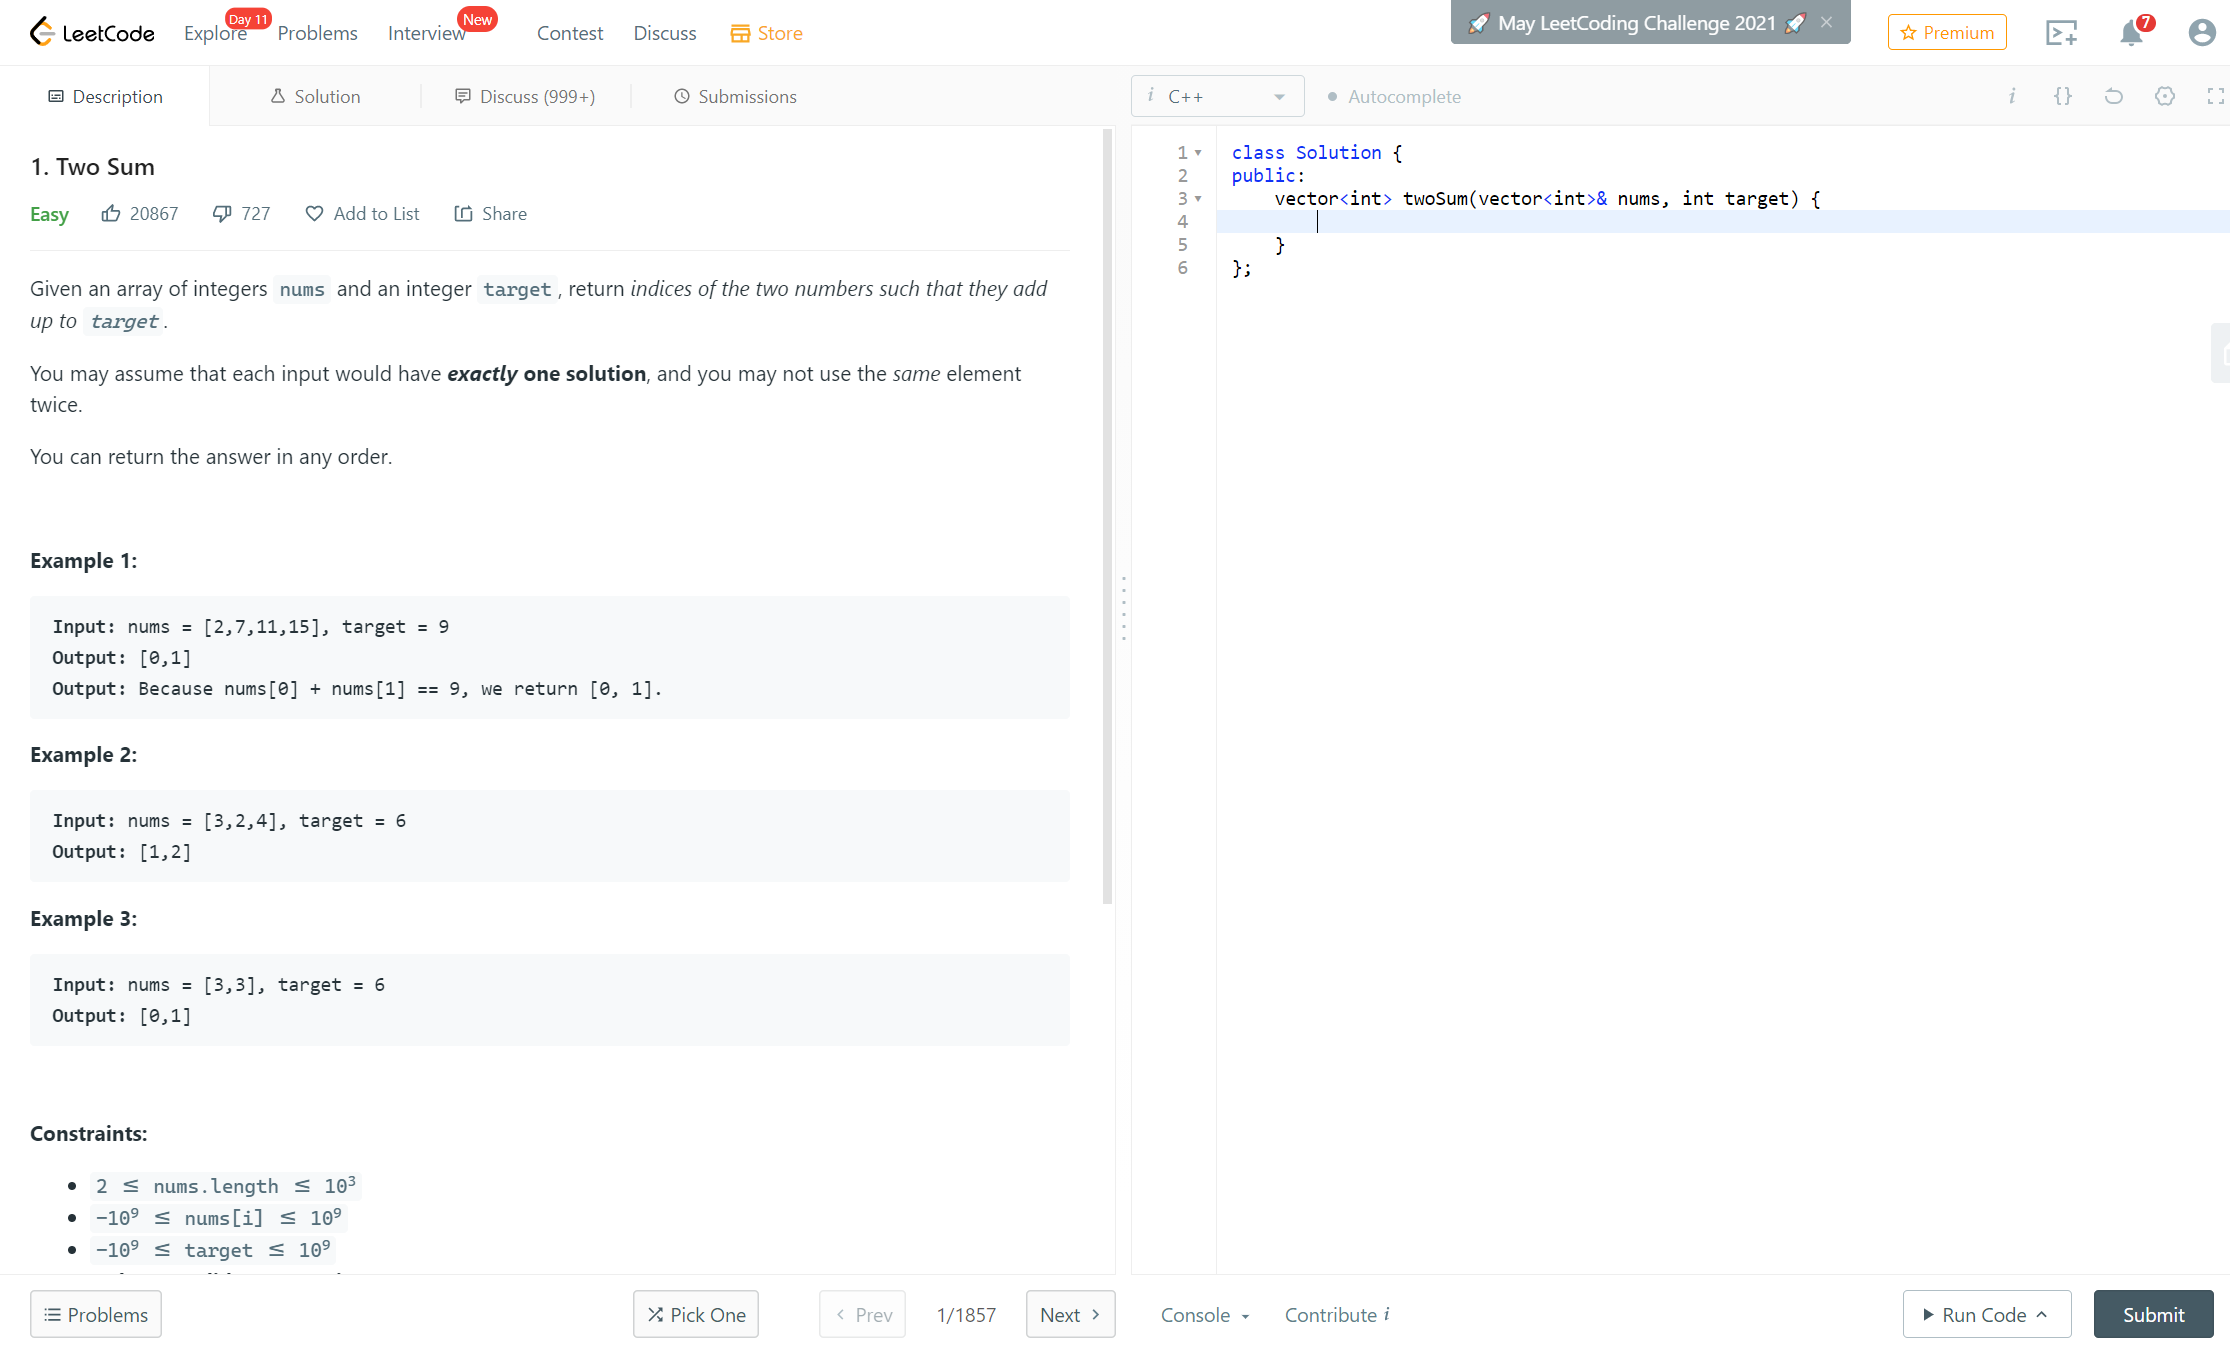
\includegraphics[width=\linewidth]{Two-Sum-LeetCode-Coding}

This is LeetCode's main coding area. The user's screen is spliteed into two parts - the question secton and the code editor for inputing answer. User can drag the splitter in the middle to adjust the size of each section.

The question section contains 4 tabs, `Description' tab displays the content of the question. `Solution' tab displays the solutions from the community. `Discuss' tab displays the discussions in the community. `Submission' tab lists user's previous submissions. Since I am not adding social functions in my solution, I will ignore the `Solution' and `Discuss' tab. Under the `Description' tab, LeetCode provides the context of the question, followed by 3 examples, and constrains for this question. The examples allow the user to run and check their solution before formal submission for marking, this can help them avoid silly mistakes. My solution should also provide similar examples for each question. Under the `Submission' tab, LeetCode records every history submission, so the user can revise old questions more efficiently. My solution should provide a similarly function as well.

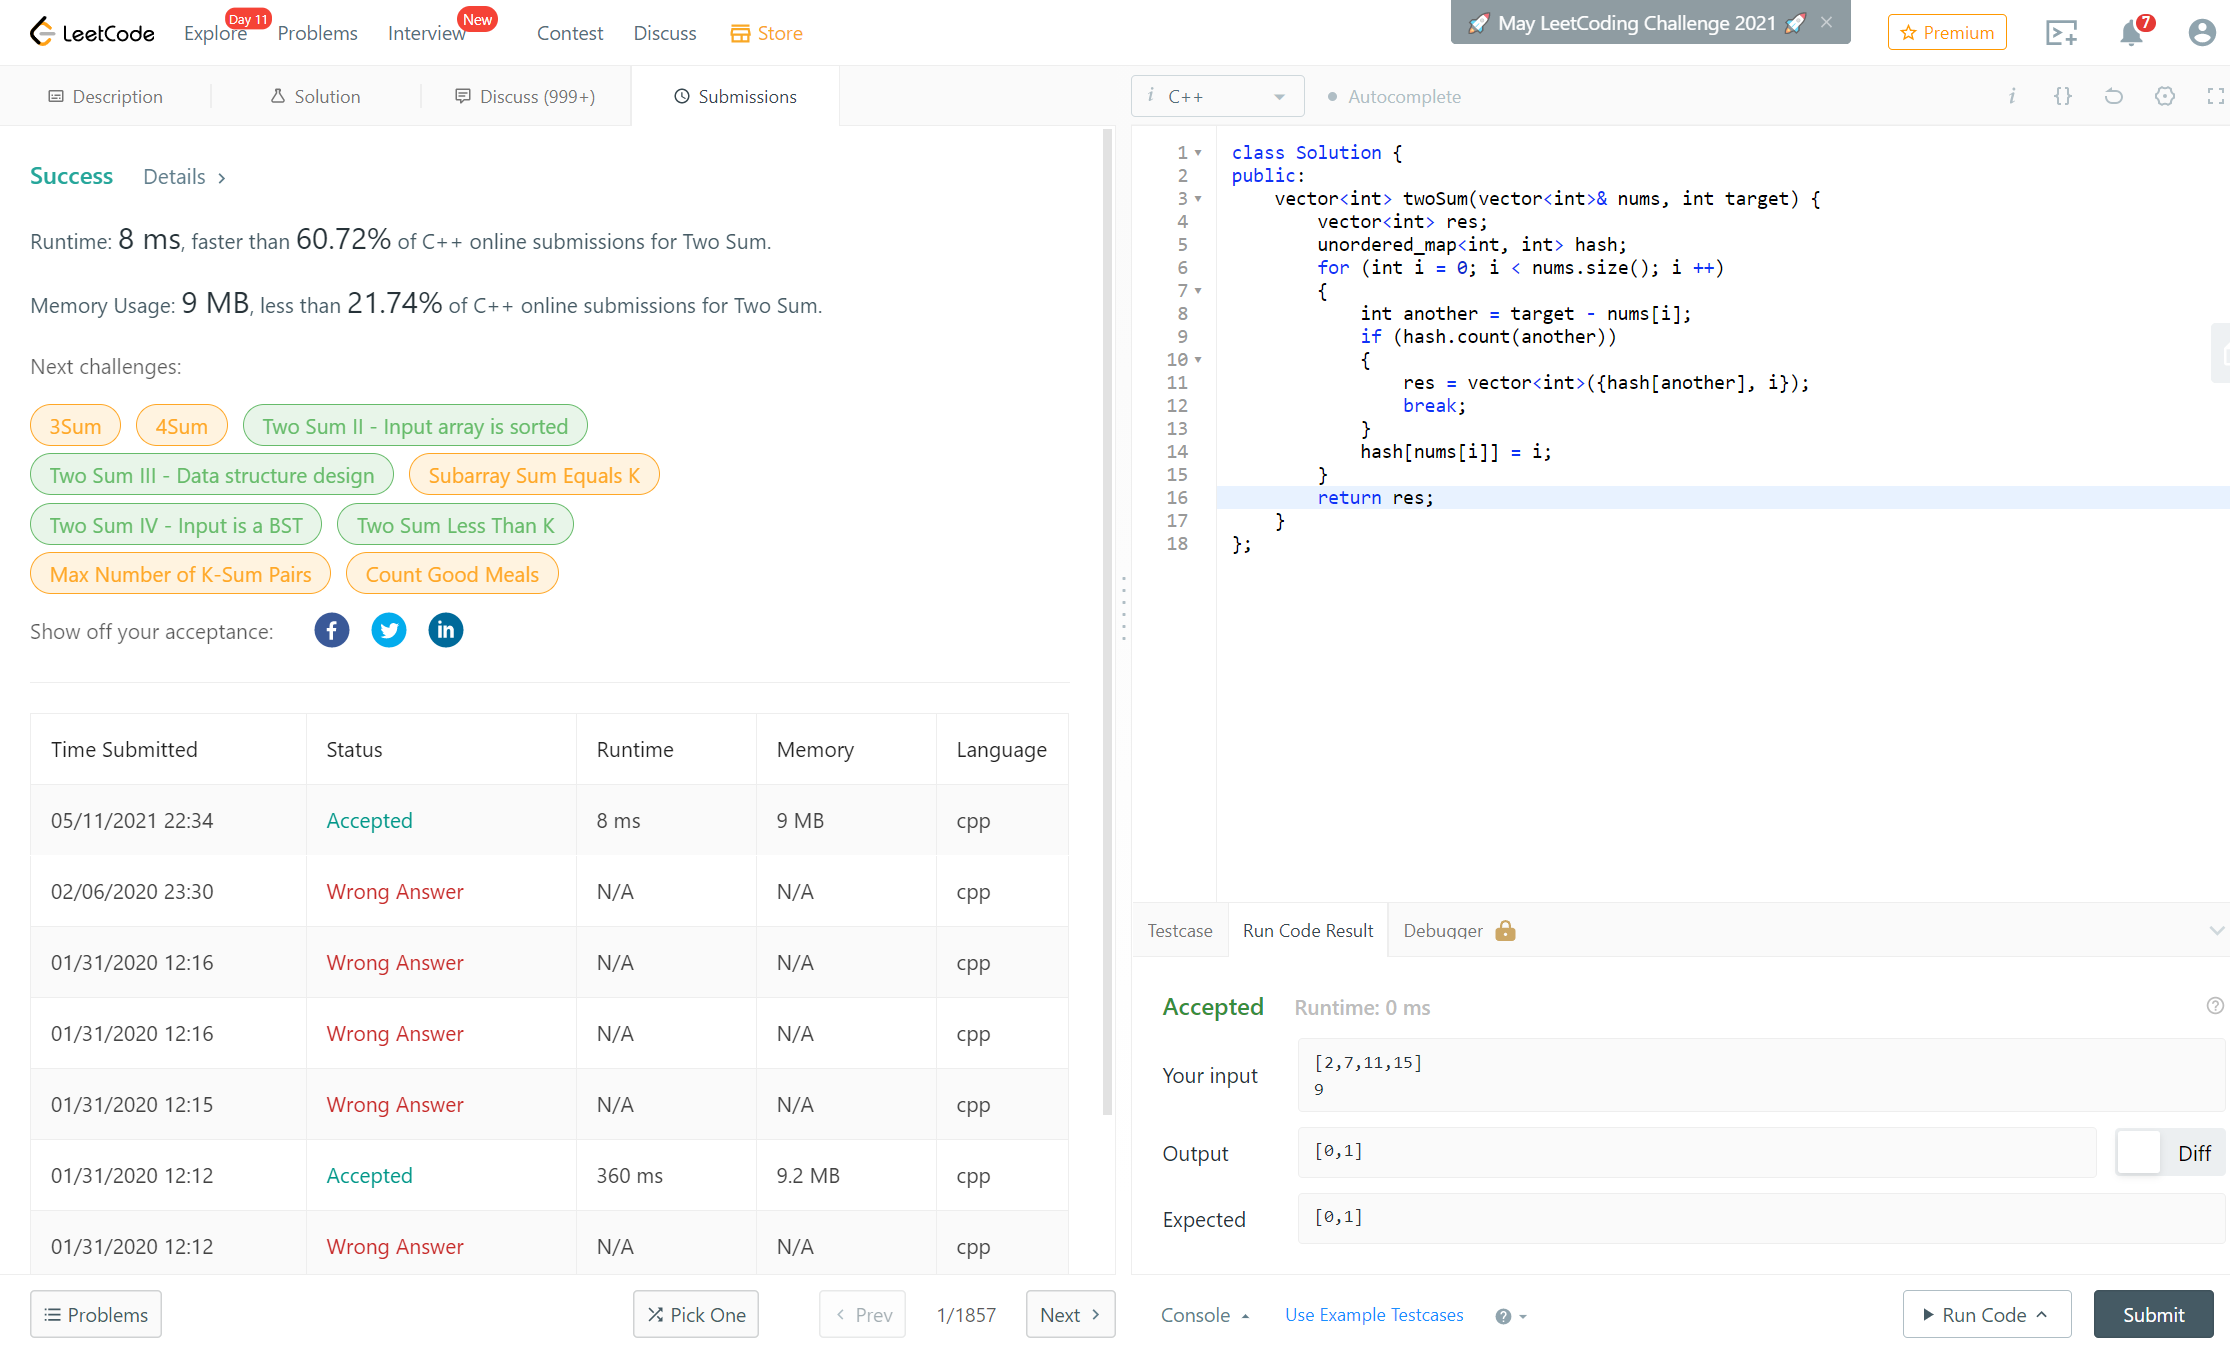
\includegraphics[width=\linewidth]{Two-Sum-LeetCode-Submission}

The code editor provides line number and syntax highlighting functions. User can change their programming language with a drop-down box. LeetCode supports all mainstream programming languages. My solution should be able to support multiple programming languages as well, which allows students with different background using it easily.

On the button, the user can `Run Code' to test their code against the examples before submission, and then click the `Submit' button to submit their solution formally.

The split view design is clean and handy. The user can see the question and write their solution on the same page without switching between different windows. The design of examples and the `Run Code' button is useful as well. I can refer to LeetCode's coding layout when designing my solution's interface.

\subsubsection{Question database}

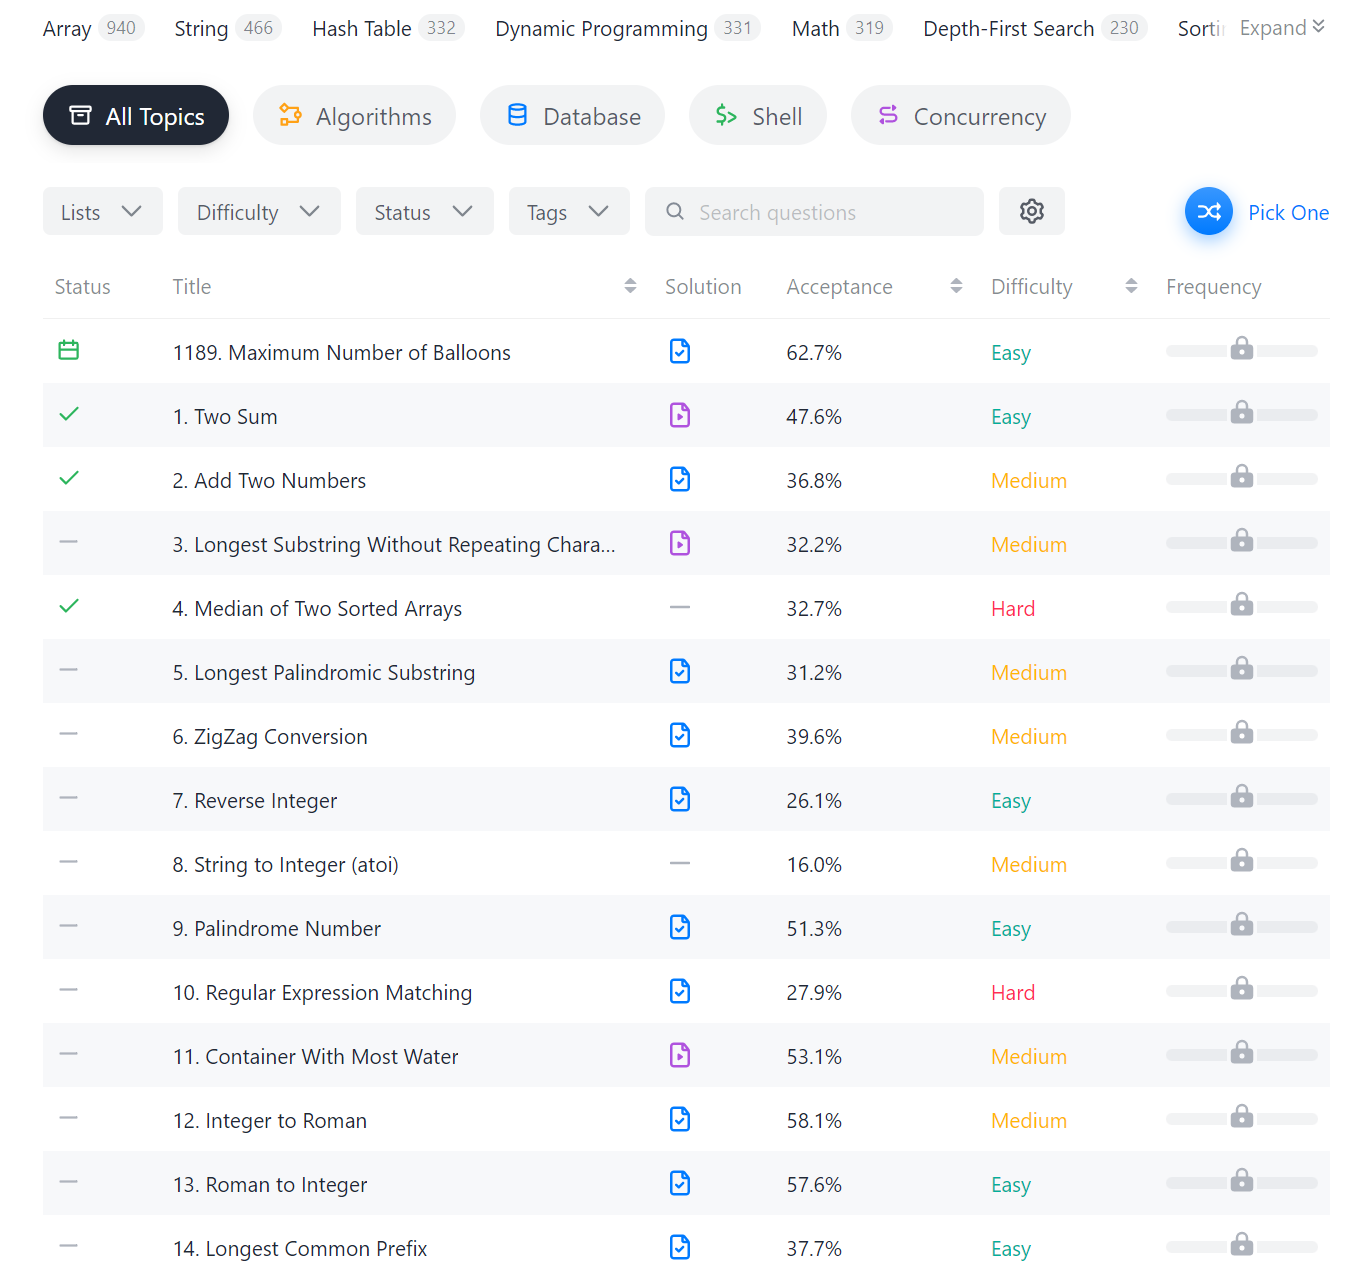
\includegraphics[width=\linewidth]{LeetCode-Problems}

Every question in LeetCode has many different attributes (Lists, Difficulty, Status, Tags, Title, Acceptance), so it is very easy for a user to find a suitable question to practice. My solution can organizes the question database in a similar way and provide corresponding query interface for a better user experience. The `Pick One' button on the top right is a very handy feature as well. User can simply click that button to start working on a quick random question. The idea of `a list of question' is great. Users can organizes a series of questions to practice and share with each other.

\subsubsection{Pricing}

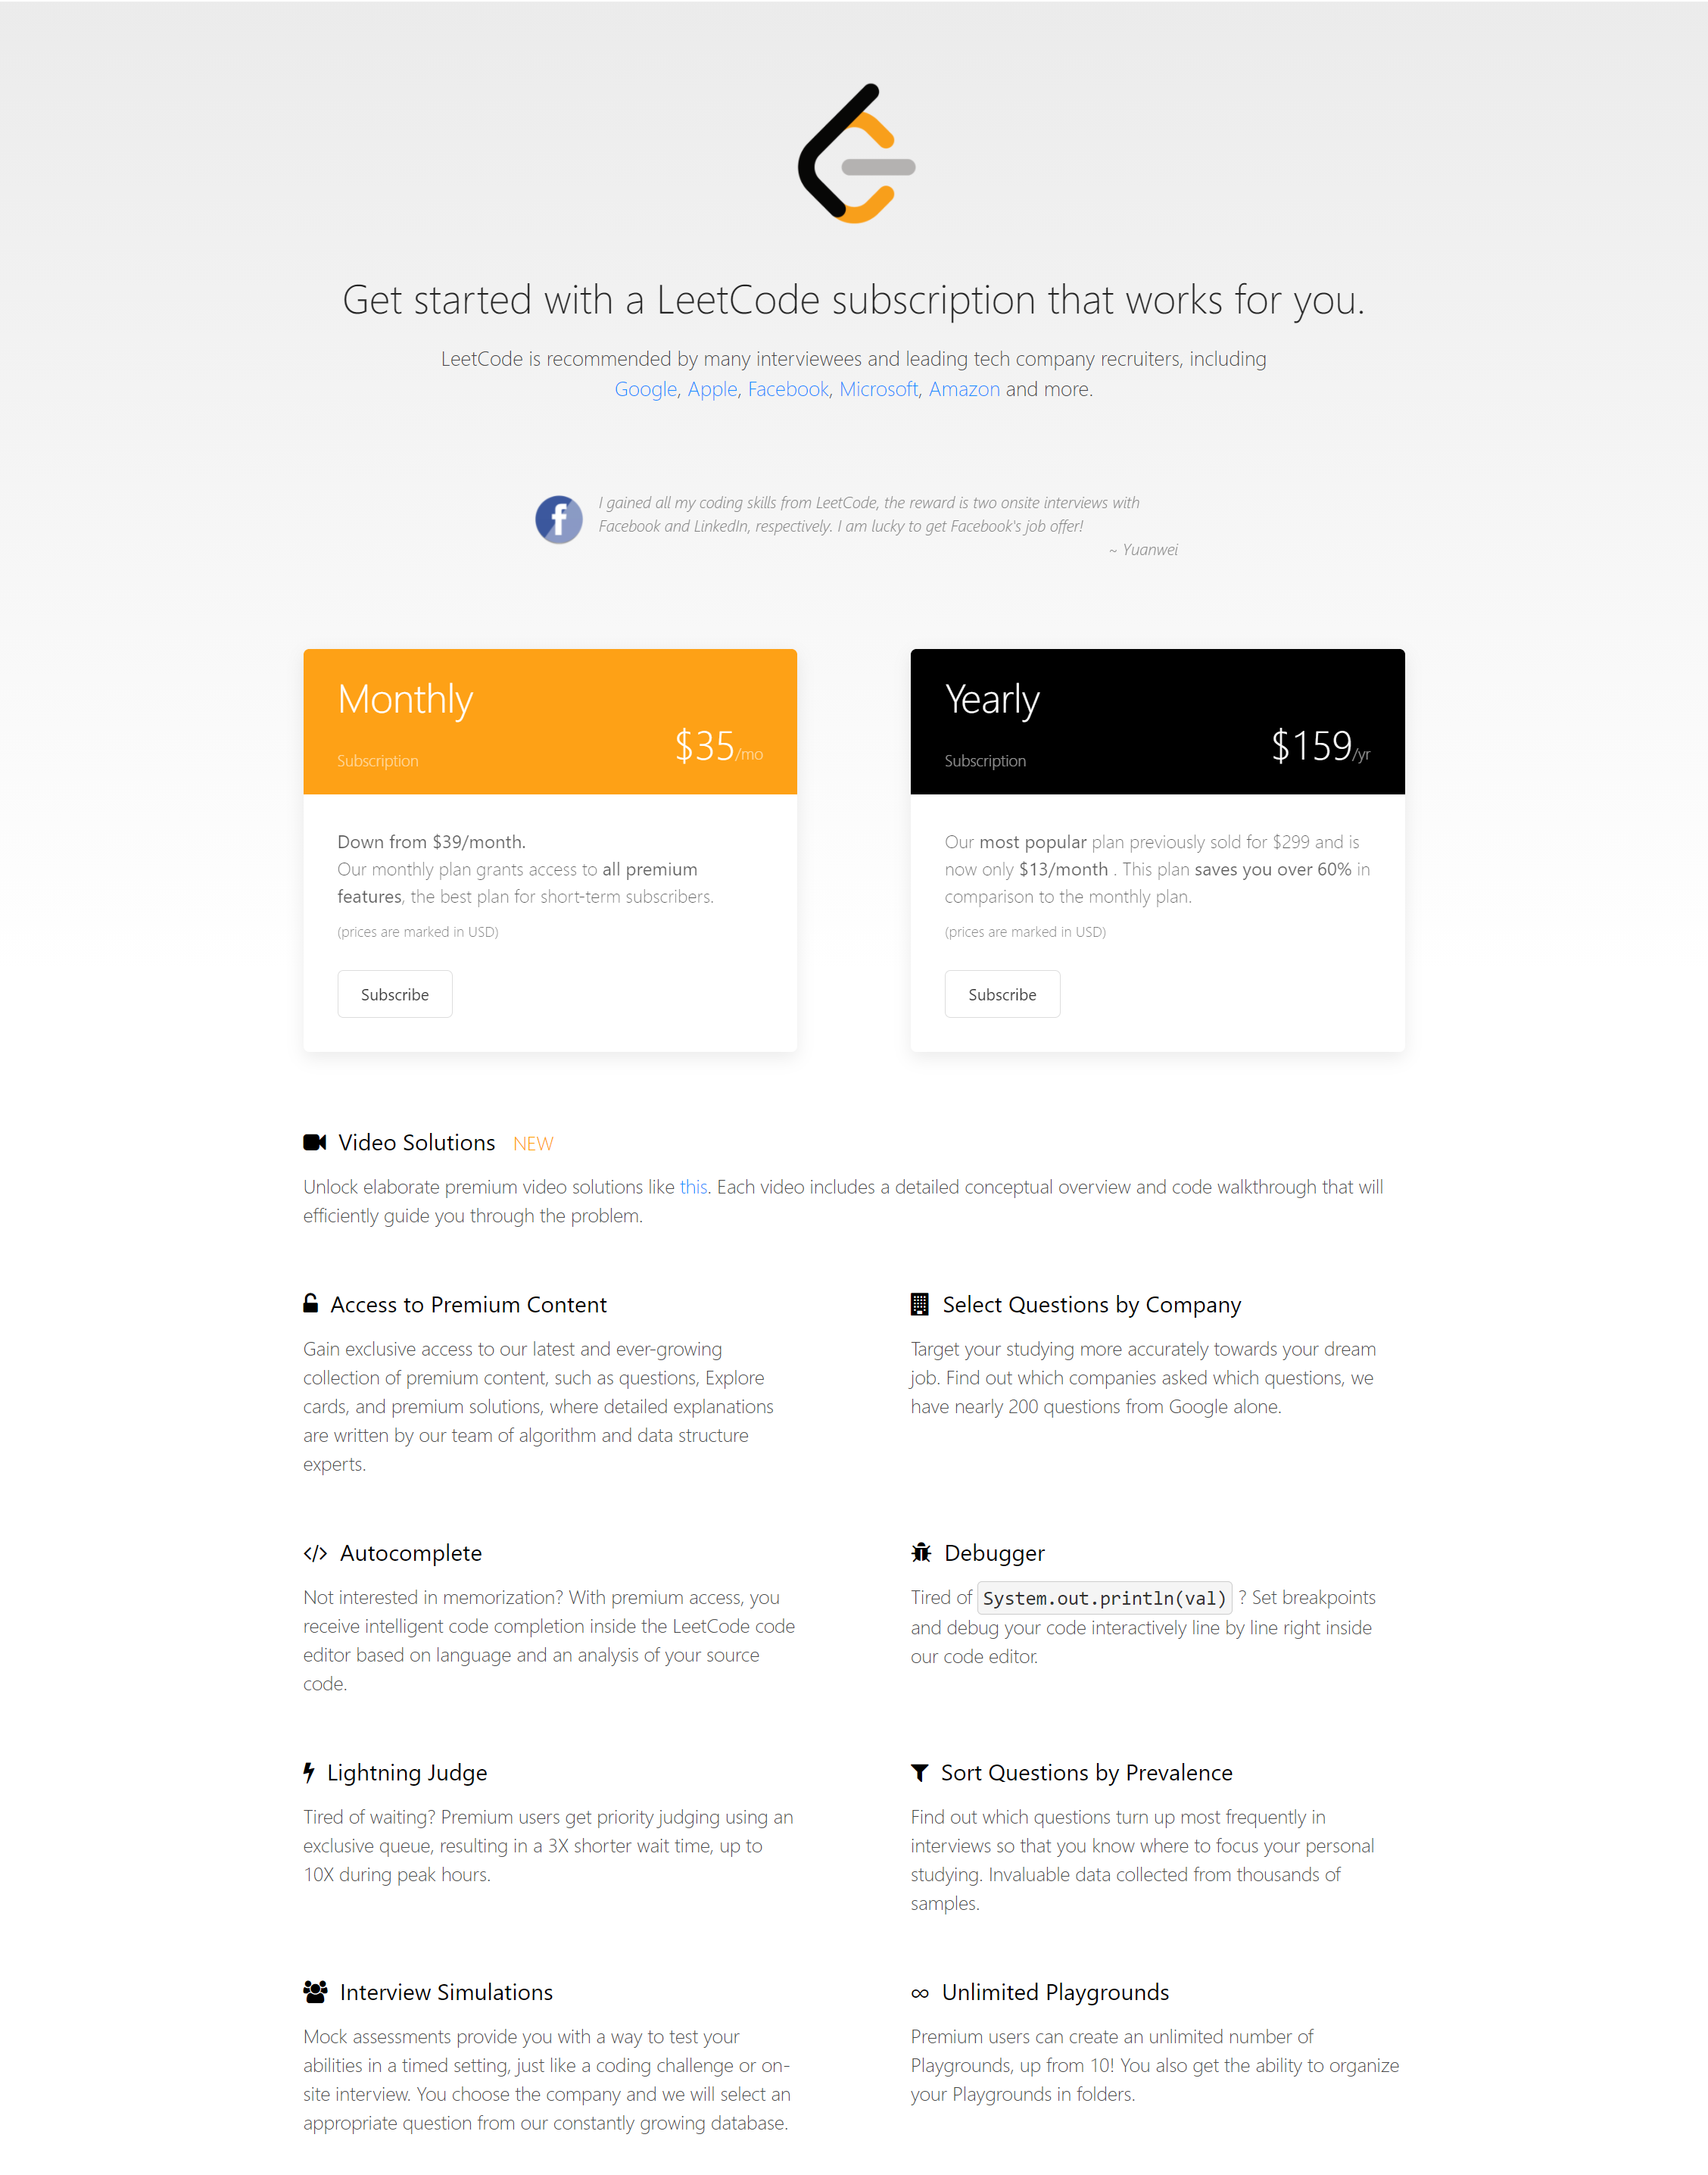
\includegraphics[width=\linewidth]{LeetCode-Premium}

The basic functions of LeetCode is free to use for all users and it charges a fee for premium subscriptions. The premium subscription provides a larger question database, better code editor, faster judger and more.

\subsubsection{Analysis}

LeetCode is a fully web-based solution, which means it works on any devices. However, it also means you will not be able to use it without an stable Internet connection. I decide to make my solution a desktop application, since most students practice coding with a computer. It also save me a lot of cost from running and maintaining a server. LeetCode runs a large community for users to discuss questions with each other. I am not adding such function to my solution. Teachers and students can use existing platforms they have been familiar with, it is unnecessary for me to develop a new platform and for the users to migrate from mature solutions. LeetCode has an easy-to-use graphical interface, which is important so new users can get their hands on very easily. 

LeetCode does not support custom questions or any functions for educators. It is mainly designed for self-learners. My solution is designed for school use, so it must support functions like custom questions, custom assignments, statistics data visualisations. LeetCode charges a subscription fee for essential functions. My solution will be free and open-source so everyone can benefit from it.

\subsection{Codeforces}

Codeforces is a competitive coding platform, it is mainly used by people to held coding competition.

\subsubsection{Main question layout}

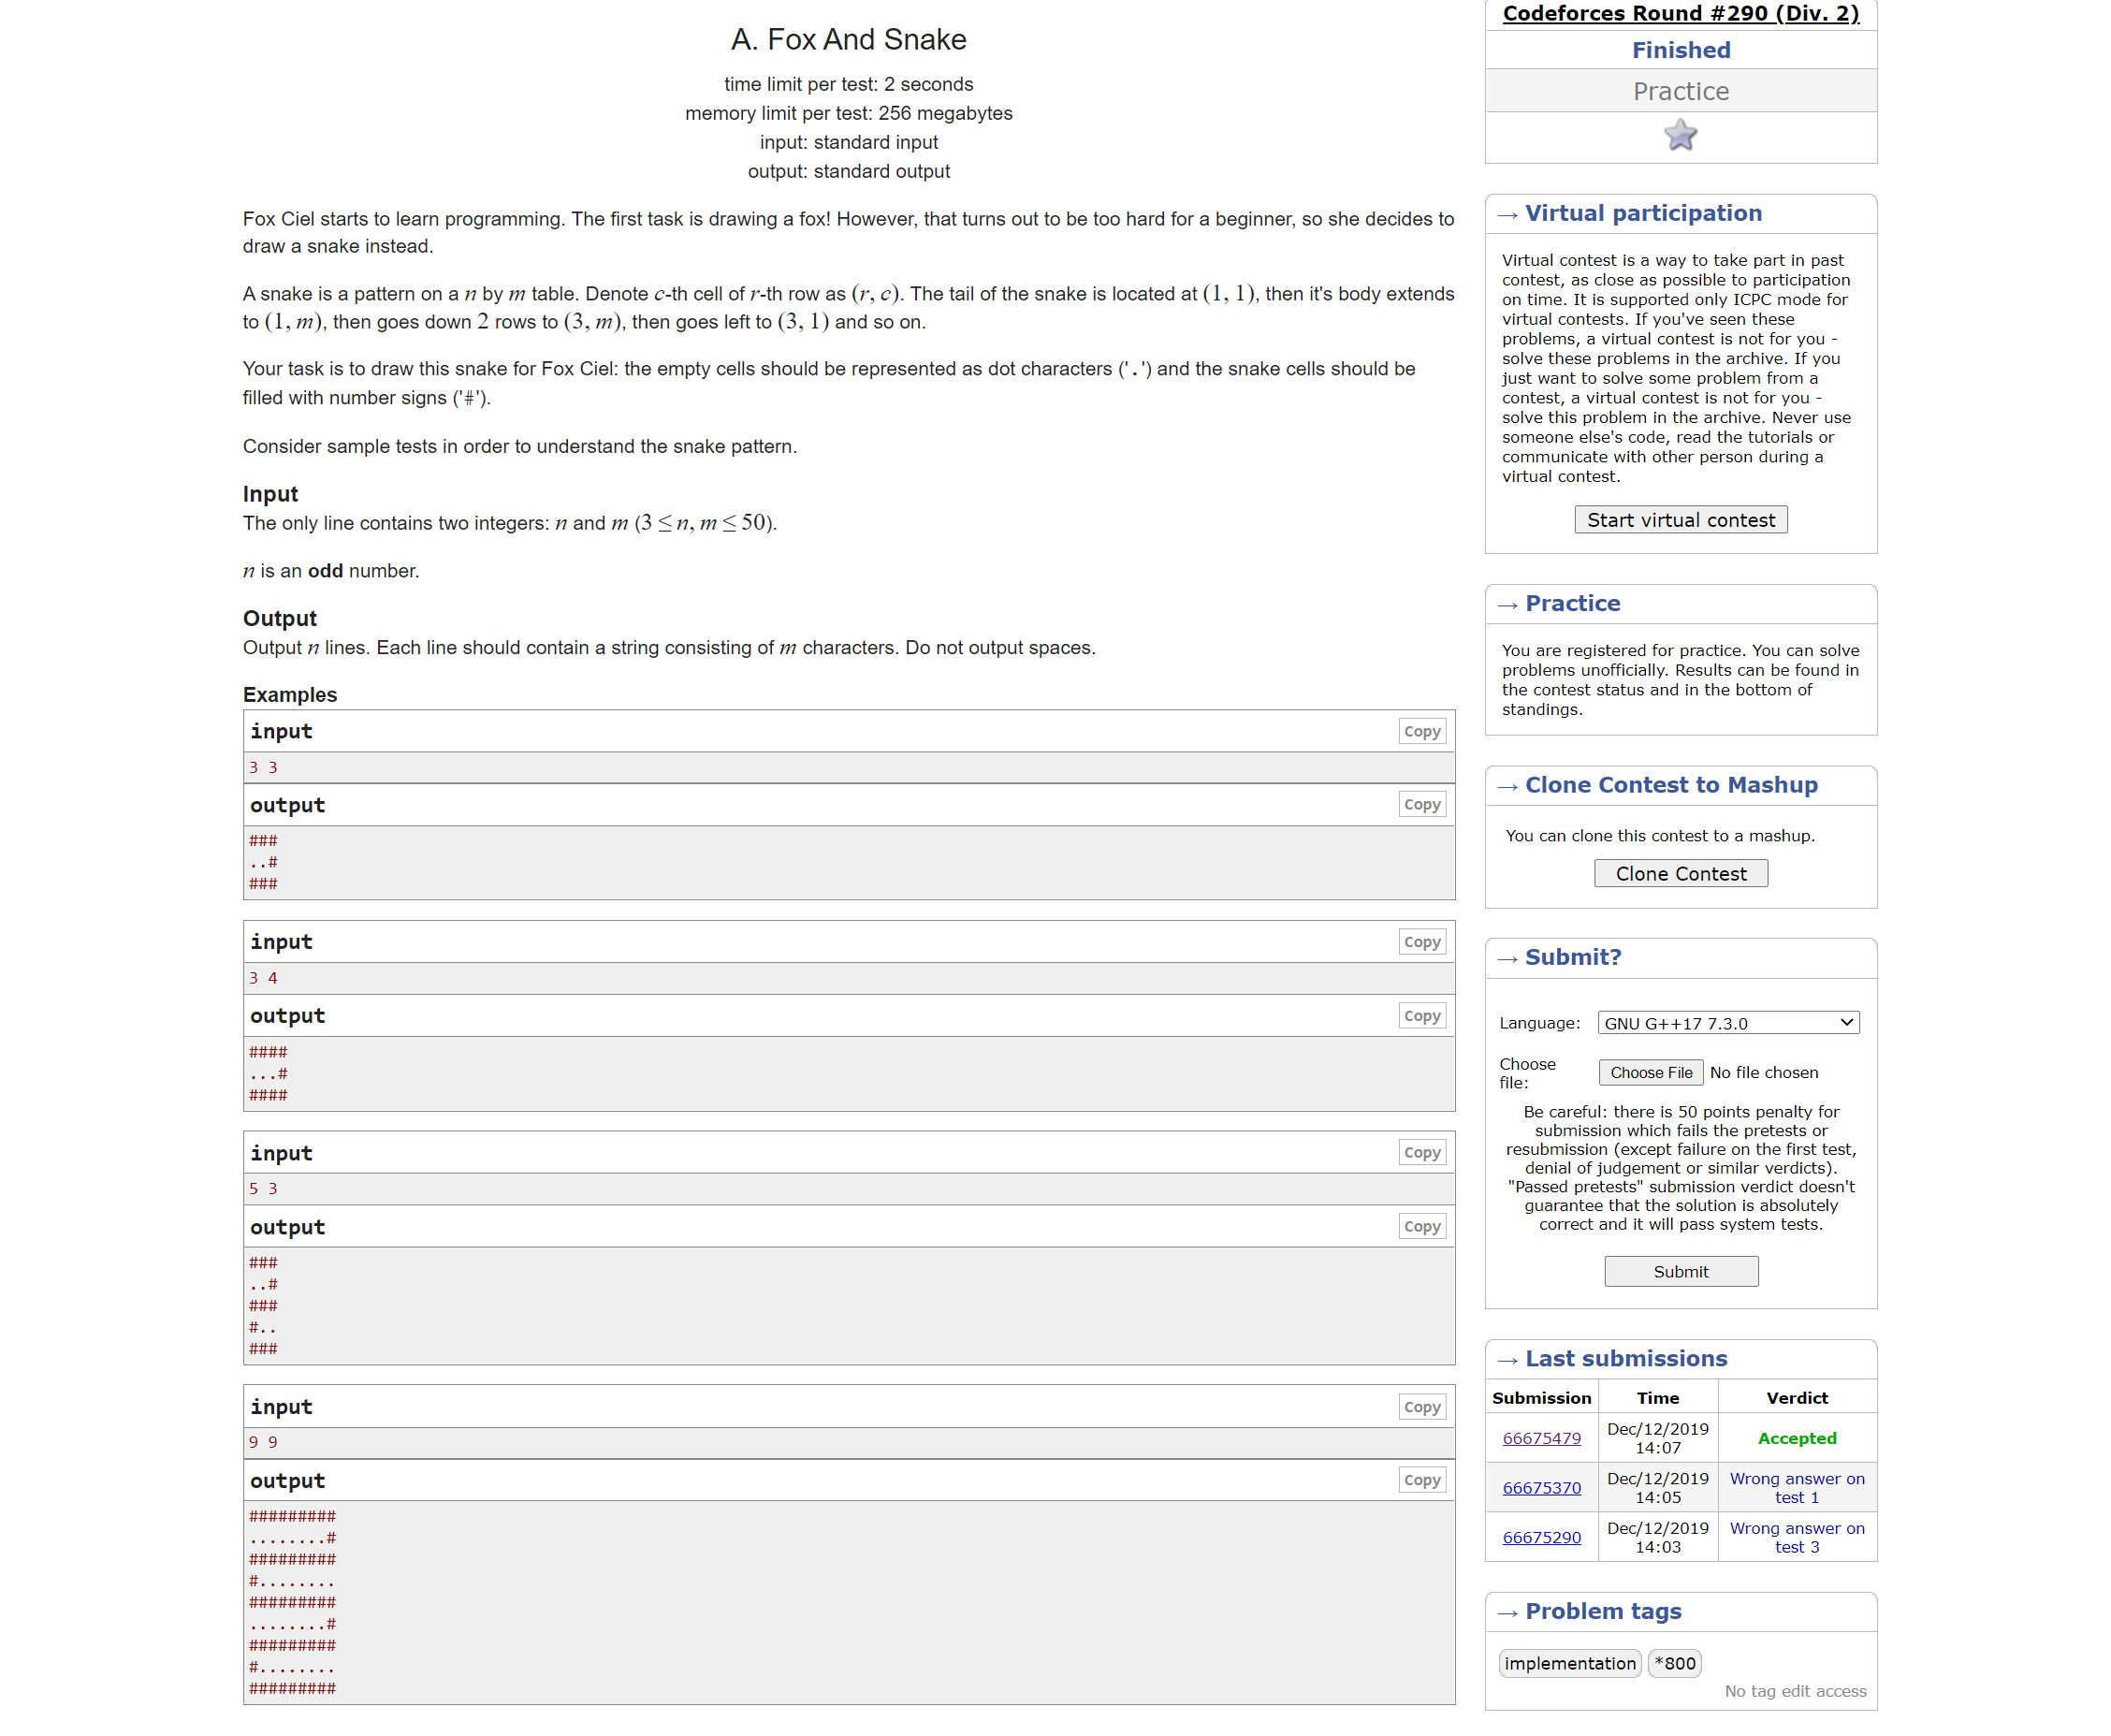
\includegraphics[width=\linewidth]{Problem-A-Codeforces}

The questions and the examples take up nearly all the spaces on the question page. There is no online editor or online runtime environment provided. Users are expected to write and test their code in their own IDEs and only submit the solution for judging. Custom IDEs may be more powerful than a builtin one. My solution will provide an editor, it is much more convenient to use. Even if a user decide to use his own environment, he can paste his code into the editor for submission. It sets time and memory limit for users' submissions, if a piece of code takes to long to run, or takes up too much memory while running, it will be terminated and marked wrong.

\subsubsection{Submission}

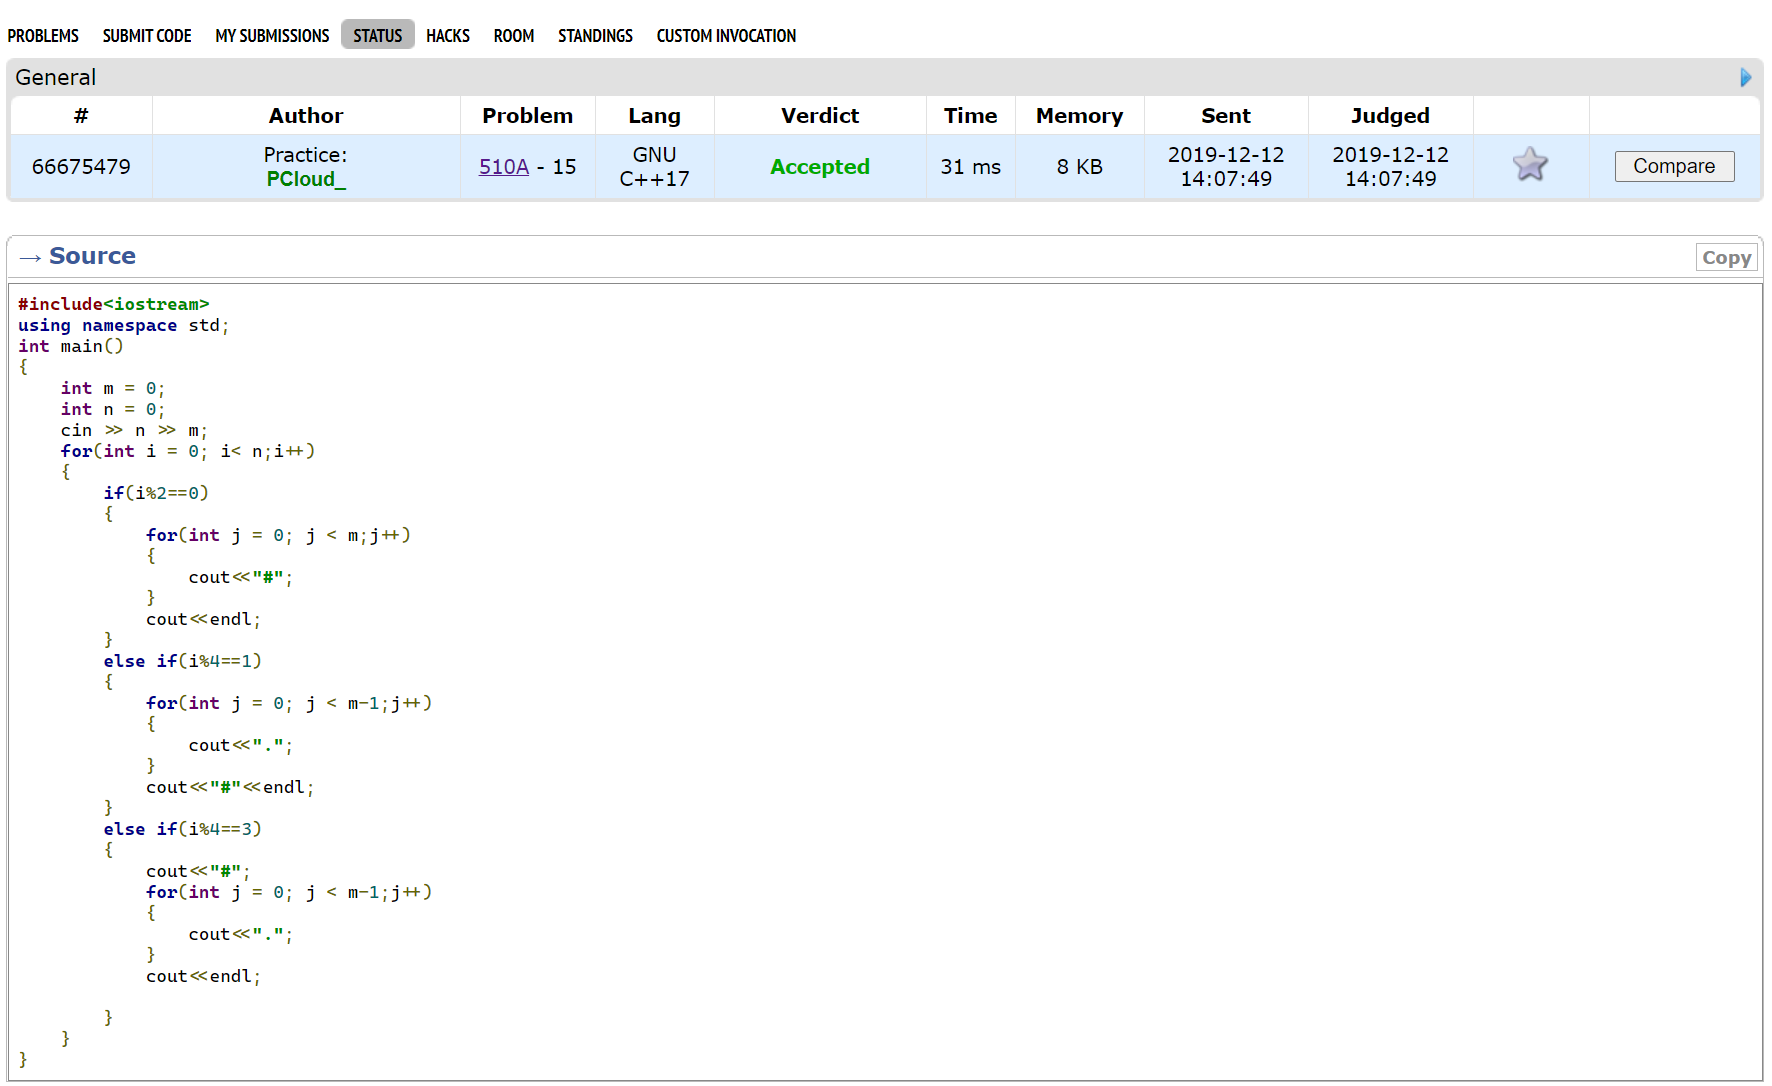
\includegraphics[width=\linewidth]{Submission-66675479-Codeforces}

When the user submits the code, the code enters a queue waiting for judging, then the user can look up their result. Users can check their source code, performance stats, and more important, when they have not passed all test cases, they are able to see what they have got wrong. The judgement protocol provide detailed information about each test case, so users can debug easily.

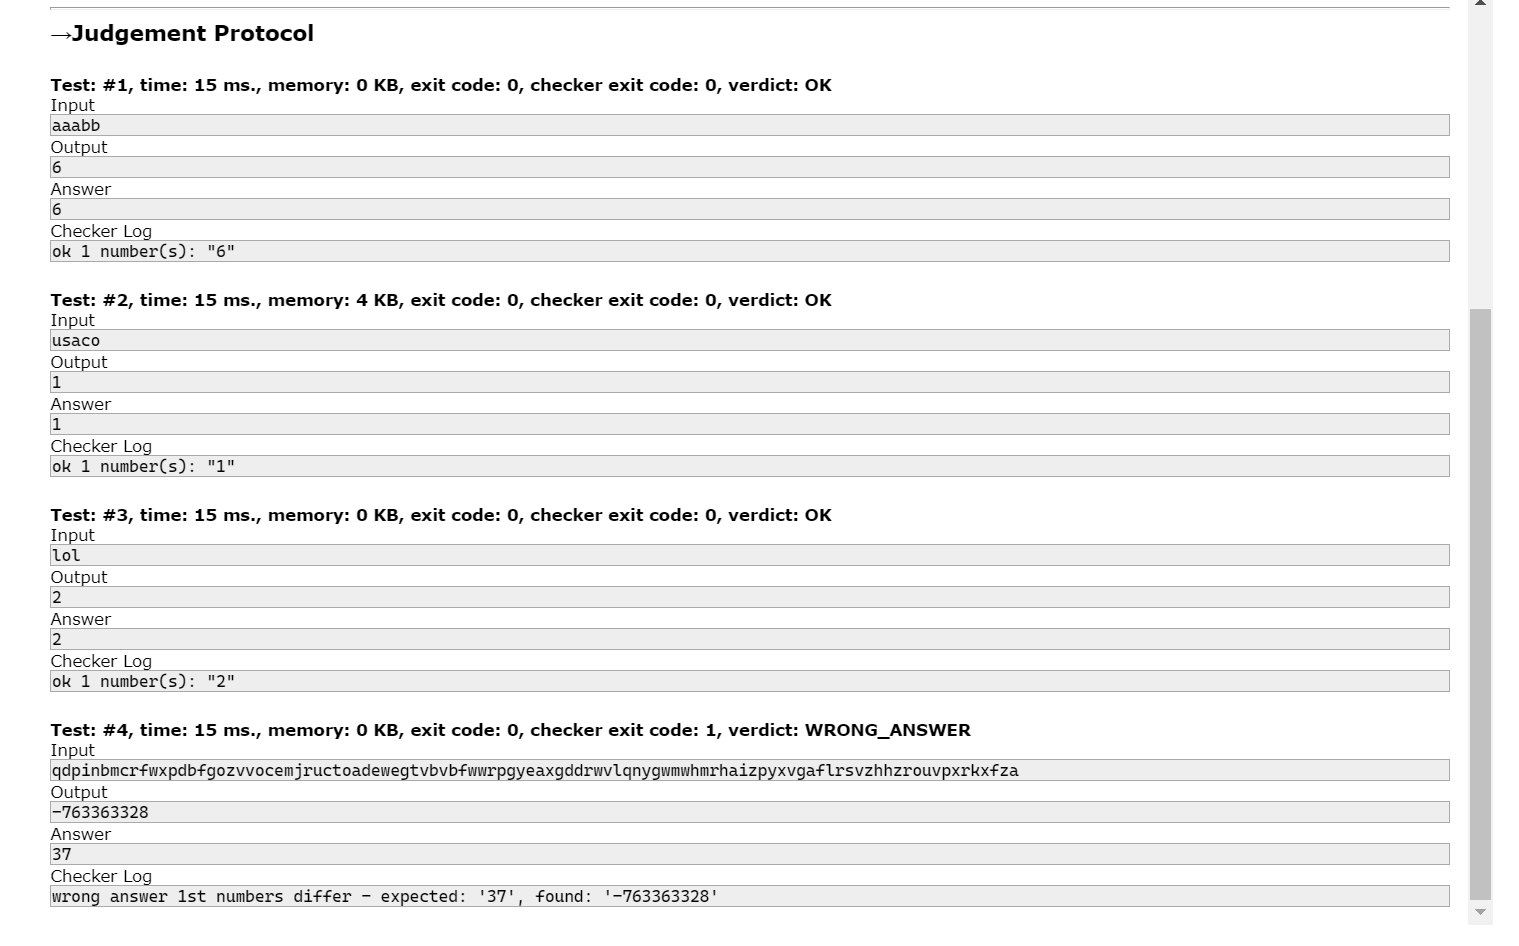
\includegraphics[width=\linewidth]{Judgement-Protocol-Codeforces}

\subsubsection{Analysis}

Codeforces is optimized for coding competition, so it has a light weight and complex interface for better performance. It is completely free to use. Users can create their own questions but it is very complicate to do so. My solution needs to enable users without experiences to create questions easily. There is no function for education - there is no way for a teacher to `create a class' and monitor his students. Codeforces is an online platform, so it also work across all devices and require an Internet connection. Users have to use their own IDEs to write and debug their code. Codeforces sends all submissions to a central `judging queue' for marking. My solution will mark all submissions in local, which makes judging a lot faster and save me from running a server. By limiting time and space allowance, Codeforces effectly prevents malicious code from running.

\section{Features}

 (TODO): Propose a solution to the problem by describing each element of the product in detail.  You can have mock ups of the graphics / screen designs from a drawing application at this stage.

\section{Limitations}

The software will be written in C\# instead of web-based which means extra software needs to be downloaded by the user. I plan to use .Net 5 runtime and WinUI 3 library for my solution, so only the Windows 10 1809 or newer Windows operating systems will be supported. This should not cause much compatibility issues since most school computers are running the required version of operating system. Downloading an extra software is inconvenient and may violate the IT security policy of some schools.

The judger can only accept code submission in limited programming languages and the user may requie to configure their own runtime environment. Creating a compiler for `OCR Pseudocode Programming Language' is too complex for this project. I will attempt to allow the user to add their own programming language and write a documentation for them to make the process easier. 

Unlike LeetCode, there is no Discussion pages for users to discuss questions because it is a desktop program instead of a web one. But this is not a big problem, students and teachers should use an existing product such as Microsoft Teams which has very good support in sharing code snippets. It is unnecessary to rebuild the wheel.

Distribute the questions and assignments is still something inconvenient. Currently, distributing questions and assignments requires the teacher to first export the questions and assignments, then send them to the students through email or file-sharing platforms. When the students finish working, they need to send their result back through email or other apps. I have attempted to integrate the file-sharing function with the existing platform - the Microsoft Teams Assignment function. \sout{But very unfortunately, the Graph API required for this operation is still in beta version, which means it can only be tested in the development environment and cannot be used in production. So for now, the users still have to use this inconvenient way to share questions and submissions. But in the future, the integration with some existing platforms may improve the experience.} (Update: the Microsoft Teams API is out of beta, now it is possible to integrate with it)

There are no good ways to maintain and distribute a large question database. Computer Science teachers are requied to maintain a database for their own students. But this is a difficult work. Creating good test cases is much time consuming than writing a mark scheme, it is very likely for a wrong solution to pass the judging if the test cases are not good enough. It relies on the teacher who creates the questions to consider everything clearly to minimize its impact.

The judger can only simply compare the students' output with the expected output, if there is a format error such as trailing space and extra newline in their output, which will not be considered as a mistake in a real exam, will be marked as a wrong answer by the judger. So students may need to spend extra time debugging their output format. It cannot judge "partially correct" answer as well. It does not care which line did the student get correct or wrong, if the final output doesn't match, the submission will be marked wrong. 

\section{Hardware and software requirements}

\begin{tabulary}{\linewidth}{|L|L|}
    \hline
    Hardware and software requirements & Justification \\
    \hline
    Standard mouse, keyboard and monitor. & Standard I/O devices are required for the user to interact with the software. Users need a mouse to navigate around different menus and pages, they need to use a keyboard to input their code solutions and use a monitor to get the output from the software. \\
    \hline
    Operating system: Windows 10 (1809 or later), Windows 11. & The software is designed with the WinUI 3 library and .Net 5 runtime, which require such operating system to run. \\
    \hline
    x86 64-bit CPU (Intel / AMD architecture) with 2 or more cores and 1 GHz or higher clock speed. & A modern CPU is required for the software. 1 core will be used to run the main program and at least 1 spare core is required for the judger to judge the submitted code. A clock speed higher than 1 GHz is required to ensure the software is running smoothly. \\
    \hline
    1GB free memory or more. & Around 512MB RAM is required to run the software, and another 512MB RAM is required for the judger to judge the submissions. \\
    \hline
    256MB free disk space or more. & 256MB free disk space is required to store and run the program itself, user may need extra disk space to store extra cache data and the database. \\
    \hline
    A modern dedicate or integrate graphics card. & The software has very little graphical demand, if the user's graphics card can run their operation system, it should be able to handle software as well. \\
    \hline
\end{tabulary}

\section{Success criteria}

\begin{tabulary}{\linewidth}{|L|L|}
      \hline
      Criteria & Justification \\
      \hline
      Provide a menu and a homepage filled with buttons link to different functions of the solution. & To make the program easy to use and allow the user finding the function they want to use quickly \\
      \hline 
      Proide an interface for the problem database. & Users can search for questions easily through the interface \\
      \hline
      Provide an interface for the user to add or export new questions. & Users can easily add new questions, edit existing questions or share them with others. \\
      \hline
      Provide a training interface where the quesiton and the code editor is displayed. & This allows the user to practice. \\
      \hline
      Provide a setting menu for the user to adjust their preferred programming languages, colour theme, and other settings. & Users can have a customzied experience with different setting options. \\
      \hline
\end{tabulary}

\chapter{Design}

\section{Decomposition}

(TODO): Add design chapter

\chapter{Development}

(TODO): Add development chapter

\chapter{Evaluation}

(TODO): Add evaluation chapter

\end{document}
